\chapter{ИССЛЕДОВАНИЕ АЛГОРИТМОВ РАСПРЕДЕЛЕНИЯ РЕСУРСОВ РАДИОКАНАЛА ПРИ АДАПТИВНОЙ ПЕРЕДАЧЕ ВИДЕОДАННЫХ}
\label{chap4}

\section{Вводные замечания}
\label{chap4:Intro}

В разделе \ref{chap3} было проведено исследование максимально возможной производительности алгоритмов распределения ресурсов радиоканала на базовой станции в беспроводных централизованных сетях для передачи неадаптивных видеопотоков. Несмотря на широкое использование неадаптивных видеоплееров для передачи видеоданных, в настоящее время все большую популярность приобретают адаптивные технологии передачи видео по протоколу HTTP (подраздел \ref{chap1:VideoPlayers}). Наиболее ярким представителем подобных технологий является стандарт Dynamic Adaptive Streaming over HTTP (DASH) \cite{dash_standard,conviva}.

Данная технология позволяет пользовательскому устройству подобрать качество видео под конкретные условия в сети передачи видеоданных. Это может привести к снижению нагрузки на сеть передачи данных за счет адаптации видеоряда.
% Исключительным качеством данной технологии является инвариантность по отношению к сети передачи информации, обеспечиваемая совместным использованием сетевых протоколов HTTP (уровень приложения) и TCP (транспортный уровень). Однако, использование настоящей технологи вносит небольшую избыточность при передаче видео из-за использования квитирования пакетов протоколом TCP.
В настоящий момент широкое распространение стандарта DASH обеспечивается его использованием сервисом хранения видеоконтента YouTube, который является крупнейшим хранилищем видеоданных в сети Интернет.

Настоящий раздел посвящен аналитическому исследованию производительности беспроводных централизованных систем передачи данных с доминированием передачи видео по протоколу прикладного уровня HTTP с возможностью его адаптации под специфичные условия в сети передачи данных. Данный раздел неотступно следует системе допущений, введенной в подразделе \ref{chap2:Assumptions}.

В начале раздела предлагается критерий качества обслуживания для адаптивных видеопотоков. Далее формулируется оптимизационная задача и предлагается нижняя граница введенного критерия по всем возможным алгоритмам распределения ресурсов беспроводного канала и адаптации видеоряда. В завершении предлагается численный пример, демонстрирующий производительность стандартных алгоритмов планирования распределения ресурсов беспроводного канала в сравнении с найденной нижней границей.

Основные результаты данного раздела опубликованы в работе \cite{8089417}.

\section{Критерии качества восприятия адаптивного видеопотока}
\label{chap4:AdaptiveQoe}

В подразделе \ref{chap3:NonAdaptiveQoe} был проведен анализ основных объективных показателей воспроизведения видеоданных, влияющих на оценку качества восприятия видеопотока и описанных ранее в подразделах \ref{chap1:VideoMOS} и \ref{chap2:VideoTrafficModel}:
\begin{itemize}
	\item Битовая скорость потока, характеризующая качество видео;
	\item Длительность буферизации, включающая в себя длительности всех начальных и повторных буферизаций во время просмотра;
	\item Гладкость воспроизведения видеоряда.
\end{itemize}
Рассмотрим каждый из них с позиции адаптивной передачи видеоданных.

Принципиальным отличием адаптивных видеоплееров от неадаптивным является наличие механизма подбора репрезентации видео в зависимости от характеристик канала передачи данных или адаптации репрезентации (подраздел \ref{chap1:VideoPlayers}). Основной целью механизма адаптации репрезентации является минимизация длительности буферизации (начальные и повторные буферизации в течении просмотра видео), так как данный фактор имеет сильное влияние на качество восприятия видео пользователем. Однако, помимо общей длительности буферизации, определяющую роль при оценке качества восприятия выполняет битовая скорость потока, характеризующая качество видеоряда (подраздел \ref{chap1:VideoMOS}). Это демонстрирует сложную взаимосвязь между битовой скоростью потока и длительностью буферизации при построении управления для адаптивных видеоплееров.

Продемонстрируем эту взаимосвязь на примере. Пусть для некоторого мобильного пользователя скорость получения данных равняется $0.65$ Мбит/с и постоянна во времени. Исходя из таблицы \ref{tab:youtubeBr}, данная скорость может обеспечить просмотр видео в качестве 360p ($0.45$ Мбит/с) без возникновения повторных буферизаций во время просмотра, или в качестве 480p ($0.7$ Мбит/с) с наличием повторными буферизаций, длительностью $5\%$ от длительности просмотра. Однако, битовая репрезентация задает верхнюю границу удовлетворенности пользователя при просмотре: для данного примера при просмотре видео в идеальных условиях (минимально возможная длительность начальной буферизации и отсутствие повторных) в качестве 360p значение MOS (методология U-vMOS) не может превышать значения 3, а для 480p~--~3.64. Следовательно, обеспечение пользователю просмотра видео в качестве 360p без повторных буферизаций не приводит к его достаточной удовлетворенности качеством обслуживания, так как пользователь считается удовлетворенным если величина MOS превышает значение 3.

Приведенный выше пример демонстрирует важную специфику организации управления полезной скоростью получения данных для адаптивных видеоплееров: \textit{безусловная минимизация общей длительности буферизации не приводит к максимизации удовлетворенности пользователя просмотром видео}. Что приводит к необходимости учета битовой скорости потока в критерии качества восприятия для адаптивных видеоплееров.

Из анализа работы адаптивных видеоплееров, проведенного в подразделе \ref{chap1:VideoPlayers}, следует, что гладкость воспроизведения видеоряда обеспечивается алгоритмом выбора репрезентации, установленном на видеоплеере и ограничено сверху некоторой величиной (подраздел \ref{chap2:VideoTrafficModel}).

Таким образом, при формировании критерия качества восприятия адаптивного видеопотока необходимо учитывать два фактора воспроизведения: длительность буферизаций и битовую скорость потока.

В настоящем разделе качество восприятия фактора длительности буферизации будет оцениваться на основе критерия отношение длительностей буферизации и просмотра (определение~\ref{def:BWTR}): $$q_i = \lim\limits_{T\rightarrow\infty} \frac{b_i^T}{w_i^T},$$
где $b_i^T$~--~общая длительность буферизации пользователя $i$ за время $T$, $w_i^T$~--~общая длительность просмотра видео пользователем $i$ за время $T$.

Данный критерий позволяет оценить удовлетворенность пользователя:
$$q_i=
\begin{cases}
0, & \text{пользователь $i$ удовлетворен просмотром}\\
\varepsilon > 0 & \text{пользователь $i$ наблюдает негативные эффекты при просмотре}\\
\end{cases}.
$$
Значение критерия качества восприятия $q_i$ обратно пропорционально удовлетворенности пользователя просмотром. Впервые критерий качества $q_i$ был рассмотрен в работе \cite{Bakin_Globecom}.

В качестве критерия качества восприятия фактора длительности буферизаций, описывающего систему в целом, было выбрано среднее значение отношение длительностей буферизации и просмотра всех пользователей в системе (\ref{eq:qMetricGoal}). На значение критерия (\ref{eq:qMetricGoal}) оказывают влияние алгоритм планирования распределения ресурсов $A$, установленный на базовой станции, и алгоритм адаптации битовой репрезентации $B$, установленный на пользовательских устройствах, принадлежащим множествам $\mathcal{A}$ и $\mathcal{B}$ соответственно (подраздел \ref{chap2:Assumptions}).

\begin{equation}
	\label{eq:qMetricGoal}
	\bar{q}\left(A, B\right)=\frac{1}{N}\left(\sum\limits_{i=1}^{N} {q_i\left(A,B\right)}\right).
\end{equation}

В отличии от критерия качетсва восприятия, представленного в подразделе \ref{chap3:NonAdaptiveQoe}, наличие адаптации видеоряда вносит более сложную зависимость качества восприятия от параметров системы. Она выражается в наличии обратной связи при взаимной работе алгоритмов $A$ и $B$: исходя из скорости получения данных обеспеченной алгоритмом $A$, алгоритм $B$ выбирает битовую скорость для заказываемых сегментов, которая влияет на загрузку беспроводного канала и скорость передачи данных.

Средняя битовая скорость видеопотока всех пользователей будет использоваться для оценки фактора качества репрезентации.

\begin{equation}
	\label{eq:rateMetricGoal}
	\overline{R}\left(A,B\right) = \frac{1}{N}\left(\sum\limits_{i=1}^{N} {\tilde{R}_i\left(A,B\right)}\right),
\end{equation}
где $\tilde{R}_i$~--~математическое ожидание битовой скорости видеопотока пользователя $i$ (подраздел \ref{chap2:InterrelationVideoParams}).

В данном подразделе был проведен анализ основных факторов, влияющих на качество восприятия адаптивного видеопотока. Результатом данного анализа является выбор двух критериев качества: среднее значение отношения длительностей буферизации и просмотра (\ref{eq:qMetricGoal}) и средняя битовая скорость видеопотока всех пользователей в системе (\ref{eq:rateMetricGoal}). На основе данных критериев будет сформирована оптимизационная задача для исследования максимальной производительности беспроводных централизованных сетей связи при передаче адаптивных видеопоследовательностей.

\section{Постановка оптимизационной задачи}
\label{chap4:AdaptiveOptimizationProblem}

В данном подразделе производится постановка и анализ оптимизационной задачи для исследования максимально возможной производительности беспроводных централизованных сетей связи при передаче адаптивных видеопоследовательностей. В подразделе \ref{chap4:AdaptiveQoe} было произведено рассмотрение факторов, влияющих на качество восприятия адаптивного видео, и выделены два основных: (\ref{eq:qMetricGoal}) и (\ref{eq:rateMetricGoal}). Настоящий подраздел построен следующим образом: в начале предлагается обобщенный критерий качества, объединяющий критерии (\ref{eq:qMetricGoal}) и (\ref{eq:rateMetricGoal}). Далее предлагается обобщенный критерия качества восприятия и предлагается оптимизационная задача. В завершении подраздела производится анализ оптимизационной задачи.

Важным выводом из подраздела \ref{chap4:AdaptiveQoe} является необходимость условной оптимизации фактора длительности буферизации: $\bar{q}\left(\mathcal{A}, \mathcal{B}\right)$, при передаче адаптивных видеопотоков. Вторым фактором, влияющим на качество восприятия, была выделена средняя битовая скорость видео по всем пользователям в системе $R_{avg}$, выступающая в роли ограничения при минимизации фактора длительности буферизации. В настоящем разделе обобщенный критерий качества обслуживания для адаптивного видеоряда вводится в следующем виде:

\begin{equation}
Q = \inf\limits_{A,B: \overline{R}\left(A,B\right) \geq R_{avg}, A \in \mathcal{A}, B \in \mathcal{B}} \overline{q}\left(A,B\right).
\label{eq:extr_param}
\end{equation}

Таким образом, целью настоящего раздела является нахождение нижней границы отношения длительностей буферизации и просмотра по всем возможным алгоритмам планирования распределения ресурсов на базовой станции $\mathcal{A}$ и алгоритмам выбора репрезентации $\mathcal{B}$, удовлетворяющих допущениям введенных в подразделе \ref{chap2:Assumptions}, таким что среднее средняя битовая скорость видеопотоков превышает величину $R_{avg}$.

Важно отметить, что в настоящем разделе используется система допущений из подраздела \ref{chap2:Assumptions} без дополнительных изменений, что позволяет использовать утверждение~\ref{lem:GeneralConstrain} в виде, представленом в подразделе~\ref{chap2:InterrelationVideoParams}. Таким образом, оптимизационная задача для критерия качества (\ref{eq:extr_param}), описывающая максимальную производительность передачи адаптивных видеопотоков в беспроводных централизованных сетях, принимает следующий вид:

\begin{equation}
\begin{array}{l}
\text{ \textbf{Минимизировать:} } \frac{1}{N}\sum\limits_{i=1}^N q_i \\
\text{ \textbf{При условии:} }\\
\begin{cases}
\sum\limits_{i=1}^{N} {\left(1-\nu^R_i\nu^C_i\right)\frac{\tilde{R}_i \tilde{C}^{-1}_i }{q_i + \gamma_i}} -1 \leq 0 \\
-\frac{1}{N}\sum\limits_{i=1}^{N}\tilde{R}_i + R_{avg} \leq 0 \\
\tilde{R}_i \in \left[R_{min}, R_{max}\right], i=\overline{1,N} \\
-q_i \leq 0,\mbox{ }i=\overline{1,N} \\
\end{cases}
\end{array}.
\label{eq:optim_problem_q}
\end{equation}

Проведем анализ задачи (\ref{eq:optim_problem_q}) на качественном уровне. В настоящей оптимизационной задаче $2N$ переменных: $q = (q_1, q_2, \ldots, q_N)$ и $\tilde{R} = (\tilde{R_1}, \tilde{R_2}, \ldots, \tilde{R_N})$. Из вида первого ограничения следует, что оптимизационная задача (\ref{eq:optim_problem_q}) относится к классу задач нелинейного программирования. Важнейшим этапом анализа оптимизационных задач, определяющим возможные методы их решения, является определение подкласса задачи нелинейного: задачи выпуклого, вогнутого или невыпуклого программирования. Завершающая часть данного подраздела посвящена именно определению подкласса задачи (\ref{eq:optim_problem_q}).

Оптимизационная задача (\ref{eq:optim_problem_q}) обладает целевой функцией линейного вида и линейными ограничениями типа неравества, исключая первое ограничение, следовательно, тип задачи будет определяться видом первого ограничения. Стоит отметить, что данное ограничение~--~это функция от $2N$ переменных. Для его анализа рассмотрим случай, когда в системе находится только один абонент ($N=1$), в данном случае число переменных уменьшается до двух. Для упрощения последующих математических выкладок в выражении (\ref{eq:GeneralConstrainOneUser}) номер абонента был опущен, так как в системе присутствует только он один.

\begin{equation}
\left(1-\nu^R\nu^C\right)\frac{\tilde{R} \tilde{C}^{-1} }{q + \gamma} -1.
\label{eq:GeneralConstrainOneUser}
\end{equation}

Определене вида функции от нескольких переменных возможно на основе матрицы Гессе \cite{convex_opt}. В зависимости вида матрицы Гессе возможно определить вид функции следующим образом: если матрица Гессе является
\begin{itemize}
	\item Положительно определенной во всех точках, то функция выпуклая;
	\item Отрицательно определенная во всех точках, то функция вогнутая;
	\item Не является знакоопределенной, то функция общего вида (невыпуклая).
\end{itemize}

Матрица Гессе $H(\cdot)$ для функции (\ref{eq:GeneralConstrainOneUser}) принимает следующий вид:
$$H(\tilde{R}, q)=
  \left[ {\begin{array}{ccc}
   0 & &-\frac{\left(1-\nu^R\nu^C\right)\tilde{C}^{-1}}{(q + \gamma)^2} \\
   & & \\
   -\frac{\left(1-\nu^R\nu^C\right)\tilde{C}^{-1}}{(q + \gamma)^2} & & \frac{\left(1-\nu^R\nu^C\right)\tilde{C}^{-1} \tilde{R}}{(q + \gamma)^3} \\
  \end{array} } \right]
$$

Так как матрица Гессе является симметричной относительно главной диагонали, то для определения ее знакоопределенности возможно использовать критерий Сильвестра: симметричная матрица является положительно определенной тогда и только тогда, когда все ее угловые миноры положительны, в случае неотрицательной определенности~--~больше или равны нулю. Отрицательная знакоопределенность симметричной матрицы задается чередованием знаков угловых миноров: отрицательный, положительный и т.д. В иных случаях матрица не является знакоопределенной \cite{convex_opt}.

Найдем значения угловых миноров $\Delta$ матрицы $H(\tilde{R}, q)$:
$$\Delta_1 = 0 \cdot \frac{\left(1-\nu^R\nu^C\right)\tilde{C}^{-1} \tilde{R}}{(q + \gamma)^3} = 0.$$
$$\Delta_2 = 0 \cdot \frac{\left(1-\nu^R\nu^C\right)\tilde{C}^{-1} \tilde{R}}{(q + \gamma)^3} - \left(-\frac{\left(1-\nu^R\nu^C\right)\tilde{C}^{-1}}{(q + \gamma)^2}\right)^2 = - \left(\frac{\left(1-\nu^R\nu^C\right)\tilde{C}^{-1}}{(q + \gamma)^2}\right)^2 < 0.$$

Так как значение $\left(1-\nu^R\nu^C\right)$ и сумма значений $q$ и $\gamma$ отличны от нуля (система допущений, подраздел \ref{chap2:Assumptions}), то значение второго углового минора ($\Delta_2$) строго отрицательно. Таким образом, основываясь на критерии Сильвестра, функция (\ref{eq:GeneralConstrainOneUser}) является функцией общего вида (невыпуклой). Следовательно, оптимизационная задача (\ref{eq:optim_problem_q}) относится к подклассу невыпуклых задач.

Критично важно отметить, что для задач невыпуклого программирования не существует стандартных методов или подходов к решению \cite{convex_opt,optimizations_methods}. Следовательно, решение оптимизационной задачи (\ref{eq:optim_problem_q}) является нетривиальной задачей. В настоящем разделе будет предложено решение данной задачи, которое будет основано на двуступенчатой оптимизации. Дальнейшая часть раздела будет построена следующим образом. На первом шаге будет представлено решение задачи выпуклого программирования на основе теоремы Каруша-Куна-Таккера (ККТ) с использованием метода \textit{<<water-filling>>}, описанного в \cite{convex_opt}. Далее будет предложен алгоритм вычисления нижней границы оптимизационной задачи (\ref{eq:optim_problem_q}), который использует решение задачи на основе теоремы ККТ.

\section{Решение вспомогательной оптимизационной задачи выпуклого программирования на основе теоремы Каруша-Куна-Таккера}
\label{chap4:KktSolution}

В настоящем подразделе представлено решение задачи выпуклого программирования при наличии ограничения типа неравенств на основе теоремы Каруша-Куна-Таккера (ККТ) \cite{convex_opt,optimizations_methods}. Представленное решение было описано в работе \cite{Bakin_Globecom}.

Рассмотрим оптимизационную задачу следующего вида:

\begin{equation}
\begin{array}{l}
\text{ \textbf{Минимизировать:} } Q^{*} = \frac{1}{N}\sum\limits_{i=1}^N q_i \\
\text{ \textbf{При условии:} }\\
\begin{cases}
\sum\limits_{i=1}^{N} {\frac{\tilde{a}_i}{q_i + \gamma_i}} - L^{*} \leq 0\\
-q_i \leq 0 , i=\overline{1,N} \\
\end{cases}
\end{array},
\label{eq:optim_problem_bakin_lemma}
\end{equation}
где $\tilde{a}_i, i=\overline{1,N}$ и $L^{*}$ являются положительными и отличными от нуля числами.

\begin{lemma}
\label{lem:bakin_lemma}
Оптимальное значение $Q^{*}$ может быть получено на основе выражения (\ref{eq:optim_problem_bakin_lemma_solution}):
\emph{
\begin{equation}
Q^{*} =
\begin{cases}
0, & \text{если} \sum\limits_{i=1}^{N} {\left(\frac{\tilde{a}_i}{\gamma_i}\right)} \leq L^{*}\\
\frac{1}{N} \sum\limits_{i=1}^{N} {\mathrm{max} \left(\sqrt{\mu_0 \tilde{a}_i N}-\gamma_i, 0\right)}, & \mathrm{иначе} \\
\end{cases},
\label{eq:optim_problem_bakin_lemma_solution}
\end{equation}
}
\emph{
где $\mu_0$~--~решение уравнения (\ref{eq:optim_problem_bakin_lemma_solution_eq}):
\begin{equation}
\sum\limits_{i=1}^{N} {\frac{\tilde{a}_i}{\mathrm{max} \left(\sqrt{\mu_0 \tilde{a}_i N}, \gamma_i\right)}} - L^{*} = 0.
\label{eq:optim_problem_bakin_lemma_solution_eq}
\end{equation}
}
\end{lemma}

\begin{proof}

Из вида первого ограничения следует, что оптимизационная задача (\ref{eq:optim_problem_bakin_lemma}) относится к классу задач нелинейного выпуклого программирования. Следовательно, могут быть выписаны условия существования минимума ККТ, и существует единственная точка на многомерной плоскости, удовлетворяющая данным условиям. Теорема ККТ позволяет свести задачу выпуклого программирования к поиску стационарной точки функции Лагранжа на множестве, определенном ограничениями на неотрицательность значений множителей Лагранжа, принадлежность решения области допустимых значений \cite{optimizations_methods}.

Для оптимизационной задачи (\ref{eq:optim_problem_bakin_lemma}) найдем функцию Лагранжа $\mathcal{L}(\cdot)$:

\begin{equation}
\mathcal{L} (\boldsymbol{q}, \boldsymbol{\mu}) = \frac{1}{N} \sum\limits_{i=1}^{N}{q_i} + \mu_0 \left[ \left(\sum\limits_{i=1}^{N} {\frac{\tilde{a}_i}{q_i + \gamma_i}}\right) - L^{*}\right] - \mu_i q_i,
\label{eq:LagrangeFucntion}
\end{equation}
где $\boldsymbol{q}=(q_1, q_2, \ldots, q_N)$ и $\boldsymbol{\mu} = (\mu_0, \mu_1, \ldots, \mu_N)$ являются векторами длины $N$ и $(N+1)$ соответственно. Вектор $\boldsymbol{\mu}$ используется для обозначения множителей Лагранжа.

На основе (\ref{eq:LagrangeFucntion}), условия существования решения задачи (\ref{eq:optim_problem_bakin_lemma}) Каруша-Куна-Таккера представлены следующей системой:
\begin{equation}
\label{eq:KKT}
\begin{cases}
\frac{1}{N} - \mu_0 \frac{\tilde{a}_i}{(q_i + \gamma_i)^2} - \mu_i = 0, i = \overline{1,N} & \boldsymbol{\mathrm{Стационарность}}\\
-q_i \leq 0, i = \overline{1,N} & \boldsymbol{\mathrm{Выполнимость \quad 1}}\\
\sum\limits_{i=1}^{N} {\frac{\tilde{a}_i}{q_i + \gamma_i}} - L^{*} \leq 0 & \boldsymbol{\mathrm{Выполнимость \quad 2}}\\
\mu_j \geq 0, j = \overline{0,N} & \boldsymbol{\mathrm{Неотрицательность}}\\
\mu_i q_i = 0, i = \overline{1,N} & \boldsymbol{\mathrm{Дополняющая \quad нежесткость \quad 1}}\\
\mu_0 \left[ \left(\sum\limits_{i=1}^{N} {\frac{\tilde{a}_i}{q_i + \gamma_i}}\right) - L^{*}\right] = 0 & \boldsymbol{\mathrm{Дополняющая \quad нежесткость \quad 2}}\\
\end{cases}
\end{equation}

Теорема ККТ утверждает, что решение оптимизационной задачи (\ref{eq:optim_problem_bakin_lemma}) удовлетворяет всем условиям, представленным в системе (\ref{eq:KKT}). Одновременно с этим, выпуклость задачи обеспечивает единственность решения настоящей системы. Важно отметить, что условия ККТ могут быть применены и к задачам невыпуклого программирования, однако, в таком случае может существовать несколько возможных решений систем, аналогичных (\ref{eq:KKT}), так как в таких задачах возможно будет существовать множество локальных экстремумов. Данный факт приводит к необходимости организации перебора по полученным решениям для поиска глобального экстремума при использовании подхода на основе условий ККТ для задач невыпуклого программирования.

В обозначениях к системе (\ref{eq:optim_problem_bakin_lemma}) использовался адаптированный перевод англоязычных терминов:
\begin{itemize}
\item \textit{<<Stationarity>>}~--~\textbf{Стационарность}. Равенство градиента функции Лагранжа нулю;
\item \textit{<<Primal feasibility>>}~--~\textbf{Выполнимость}. Ограничения типа неравенства в каноническом виде;
\item \textit{<<Dual feasibility>>}~--~\textbf{Неотрицательность}. Ограничение на положительность значений множителей Лагранжа;
\item \textit{<<Complimentary slackness>>}~--~\textbf{Дополняющая нежесткость}.
\end{itemize}

Продолжим рассмотрение условий существования экстремума (\ref{eq:optim_problem_bakin_lemma}). Из условия \textbf{Стационарность} выразим значение $\mu_i$:
$$\mu_i = \frac{1}{N} - \mu_0 \frac{\tilde{a}_i}{(q_i + \gamma_i)^2}, i = \overline{1,N}.$$

Следовательно, условие \textbf{Дополняющая нежесткость 1} преобразуется к виду:
\begin{equation}
q_i \left[\frac{1}{N} - \mu_0 \frac{\tilde{a}_i}{(q_i + \gamma_i)^2}\right] = 0, i = \overline{1,N}.
\label{eq:interStep1}
\end{equation}
Уравнение (\ref{eq:interStep1}) задает зависимость значений $q_i$ от значения только одного множителя Лагранжа $\mu_0$. Проведем последовательный анализ выражения (\ref{eq:interStep1}) для конкретного пользователя $i$ в зависимости от значений $\mu_0$.

Пусть $\mu_0 \in \left[0, \frac{\gamma_i^2}{\tilde{a_i N}}\right)$, тогда выражение $\left[\frac{1}{N} - \mu_0 \frac{\tilde{a}_i}{(q_i + \gamma_i)^2}\right]$, равное $\mu_i$, принимает значения строго больше нуля. Следовательно, при данных значениях $\mu_0$, выражение (\ref{eq:interStep1}) имеет единственное решение $q_i = 0$.

Если $\mu_0 \in \left[\frac{\gamma_i^2}{\tilde{a_i N}},\infty\right)$, то значение в квадратных скобках (\ref{eq:interStep1}), равное $\mu_i$, принимает отрицательное значение при $q_i = 0$, однако, в соответствии с условием \textbf{Неотрицательность}, $\mu_i \geq 0$. Следовательно, при данных значениях $\mu_0$ решением уравнения (\ref{eq:interStep1}) является $q_i = \sqrt{\mu_0 \tilde{a}_i N}-\gamma_i$. Объединяя два полученных выше результата анализа, решение уравнения (\ref{eq:interStep1}) определяется следующим выражением:

\begin{equation}
q_i  = \mathrm{max} \left(\sqrt{\mu_0 \tilde{a}_i N}, \gamma_i \right).
\label{eq:SolutionStep1}
\end{equation}

Таким образом, задача нахождения значений вектора $\boldsymbol{q}$ может быть сведена к нахождению одного значения множителя Лагранжа $\mu_0$. Значение $\mu_0$ может быть получено из решения условия \textbf{Дополняющая нежесткость 2}, подставив в него (\ref{eq:SolutionStep1}) получим следующее уравнение:
$$\mu_0 \left[\sum\limits_{i=1}^{N} {\frac{\tilde{a}_i}{\mathrm{max} \left(\sqrt{\mu_0 \tilde{a}_i N}, \gamma_i\right)}} - L^{*}\right] = 0.$$

Данное уравнение имеет два возможных решения:
\begin{itemize}
	\item $\mu_0 = 0$. В данном случае $\forall i: q_i = 0$, если при данных значениях вектора $\boldsymbol{q}$ выполняется условие \textbf{Выполнимость 2}.
	\item $\mu_0$ находится из решения уравнения (\ref{eq:optim_problem_bakin_lemma_solution_eq}).
\end{itemize}
Настоящий факт завершает доказательство.
\end{proof}

Описанный подход нахождения решения системы условий существования экстремума в англоязычной литературе известен под названием \textit{water-filling} и представлен в \cite{convex_opt}.

Обобщая сказанное выше, решение оптимизационной задачи (\ref{eq:optim_problem_bakin_lemma}) может быть получено из решения уравнения (\ref{eq:optim_problem_bakin_lemma_solution_eq}). Важно отметить, что (\ref{eq:optim_problem_bakin_lemma_solution_eq}) обладает монотонной завистью от значения $\mu_0$. Для нахождения решения данного уравнения может быть предложена двухэтапная численная процедура (алгоритм \ref{alg:algorithm_numerical_solution}).

\begin{algorithm}
  \caption{: Численное решение уравнения (\ref{eq:optim_problem_bakin_lemma_solution_eq})}
	\label{alg:algorithm_numerical_solution}
  \begin{algorithmic}[1]
	 \item Найти отрезок $[k,r]:\begin{cases}
		\sum\limits_{i=1}^{N} {\frac{\tilde{a}_i}{\mathrm{max} \left(\sqrt{k \tilde{a}_i N}, \gamma_i\right)}} \geq L^{*} \\
		\sum\limits_{i=1}^{N} {\frac{\tilde{a}_i}{\mathrm{max} \left(\sqrt{r \tilde{a}_i N}, \gamma_i\right)}} \leq L^{*}
		\end{cases}.$
		\newline
		алгоритмом экспоненциального шага: удвоение значения $r$, до тех пор пока не найдется значение, удовлетворяющее условиям.
	 \item Найти решение уравнения (\ref{eq:optim_problem_bakin_lemma_solution_eq}) на отрезке $[k,r]$ алгоритмом дихотомии (деления отрезка пополам).
  \end{algorithmic}
\end{algorithm}
Графическое представление алгоритма \ref{alg:algorithm_numerical_solution} приведено на рисунке \ref{fig:numerical_alg}.

\begin{figure}[htbp]
\begin{center}
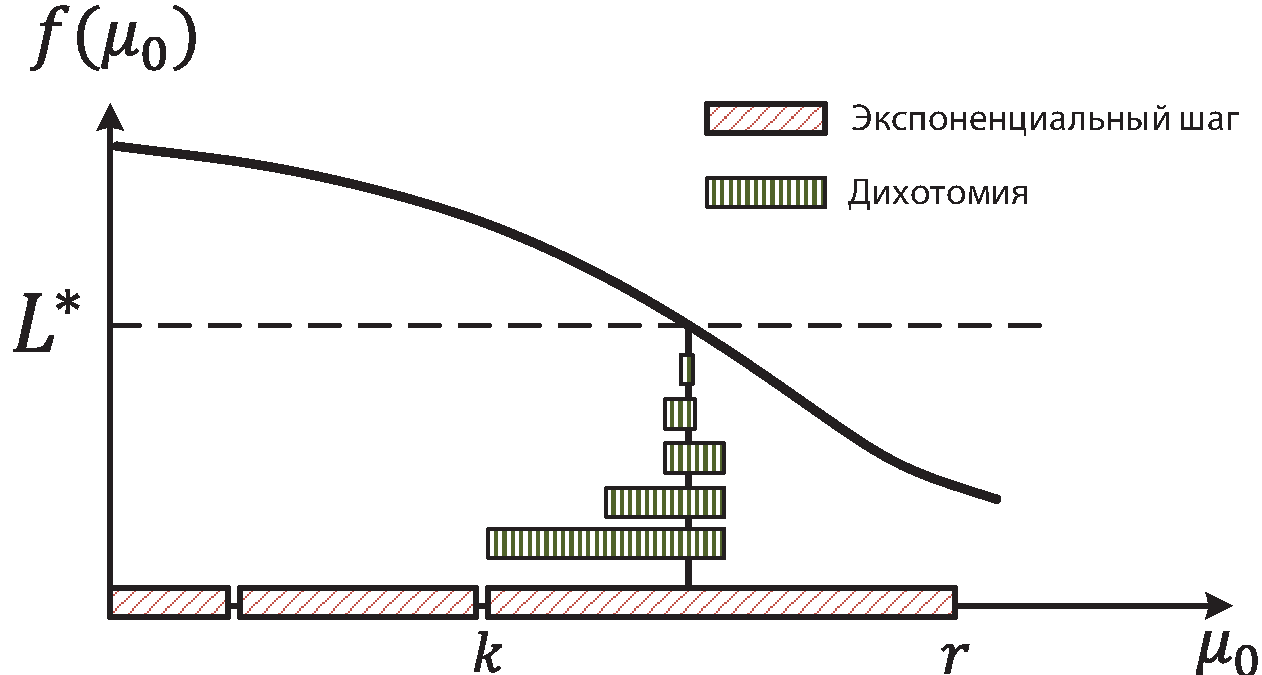
\includegraphics[width=0.7\textwidth]{Chapter4/numerical_alg.pdf}
\caption{Графическое представления алгоритма численного нахождения решения}
\label{fig:numerical_alg}
\end{center}
\end{figure}

Следующим этапом рассмотрения решения оптимизационной задачи (\ref{eq:optim_problem_bakin_lemma}) является оценка сложности полученного решения. Численный алгоритм \ref{alg:algorithm_numerical_solution} обладает логарифмической сложностью от требуемой точности нахождения решения уравнения (\ref{eq:optim_problem_bakin_lemma_solution_eq}) \cite{convex_opt, Bakin_Globecom}. На основе данного факта справедливо следующее: сложность алгоритма \ref{alg:algorithm_numerical_solution}, нахождения решения оптимизационной задачи (\ref{eq:optim_problem_bakin_lemma}), является сопоставимой со сложностью алгоритма \ref{alg:algorithm_lemma}: $O(N log_2 N), N \to \infty$ (подраздел \ref{chap3:GeneralizedFKSP}, таблица \ref{tab:nonadaptiveComplexity}).

\section{Нижняя граница отношения длительностей буферизации и просмотра при передаче адаптивных видеопотоков}
\label{chap4:LowerBoundForQ}
В подразделе \ref{chap4:AdaptiveOptimizationProblem} была предложена оптимизационная задача невыпуклого программирования (\ref{eq:optim_problem_q}), определяющая максимально возможную производительность беспроводных централизованных систем для передачи адаптивных видеопотоков. Данная оптимизационная задача учитывает два основных фактора, влияющие на качество восприятия адаптивного видео: отношение длительностей буферизации и просмотра ($q_i$) и средняя битовая скорость просмотренного видео ($\tilde{R}_i$), представленные в подразделе \ref{chap4:AdaptiveQoe}. Сложность получения решения задачи (\ref{eq:optim_problem_q}) обусловлена невыпуклостью ее ограничения, что приводит к отсутствию стандартных методов и подходов к решению. Оптимизационная задача (\ref{eq:optim_problem_q}) имеет следующий вид:

$$\begin{array}{l}
\text{ \textbf{Минимизировать:} } \frac{1}{N}\sum\limits_{i=1}^N q_i \\
\text{ \textbf{При условии:} }\\
\begin{cases}
\sum\limits_{i=1}^{N} {\left(1-\nu^R_i\nu^C_i\right)\frac{\tilde{R}_i \tilde{C}^{-1}_i }{q_i + \gamma_i}} -1 \leq 0 \\
-\frac{1}{N}\sum\limits_{i=1}^{N}\tilde{R}_i + R_{avg} \leq 0 \\
\tilde{R}_i \in \left[R_{min}, R_{max}\right], i=\overline{1,N} \\
-q_i \leq 0,\mbox{ }i=\overline{1,N} \\
\end{cases}
\end{array}.$$

Предлагаемый подход для решения задачи (\ref{eq:optim_problem_q}) состоит в разделении ее решения на два этапа.

На первом этапе будет рассмотрена промежуточная задача (\ref{eq:optim_problem_lemma_q_first}):

\begin{equation}
\begin{array}{l}
\text{ \textbf{Максимизировать:} } L = \sum\limits_{i=1}^N l_i \\
\text{ \textbf{При условии:} }\\
\begin{cases}
\sum\limits_{i=1}^{N} {l_i \tilde{R}_i - 1} \leq 0\\
-\frac{1}{N}\sum\limits_{i=1}^{N}\tilde{R}_i + R_{avg} \leq 0 \\
l_i \in \left[0, \frac{\left(1-\nu^R_i\nu^C_i\right)\tilde{C}^{-1}_i }{\gamma_i}\right] , & i=\overline{1,N} \\
\tilde{R}_i \in \left[R_{min}, R_{max}\right] , & i=\overline{1,N} \\
\end{cases}
\end{array}.
\label{eq:optim_problem_lemma_q_first}
\end{equation}

Оптимизационная задача (\ref{eq:optim_problem_lemma_q_first}) является задачей с линейной целевой функцией и одним невыпуклым ограничением квадратичного вида. Важным отличием оптимизационной задачи (\ref{eq:optim_problem_lemma_q_first}) от (\ref{eq:optim_problem_q}) состоит в виде первого ограничения: ограничение в задаче (\ref{eq:optim_problem_q}) является \textit{ограничением общего вида} (подраздел \ref{chap4:AdaptiveOptimizationProblem}), когда ограничение в задаче (\ref{eq:optim_problem_q}) является \textit{ограничением квадратичного вида}. Это небольшое отличие оптимизационных задач, имеет колоссальное влияние на методику решения. Для задач квадратичного программирования, с невыпуклым ограничением квадратичного вида существует эффективный алгоритм решения, построенный на основе метода многогранной аппроксимации (в англоязычной литературе \textit{<<polyhedral underestimating method>>}), в сочетании со стандартными численными методами решения задач выпуклого программирования \cite{Zheng2011}. Описание данного численного метода решения задач квадратичного программирования с невыпуклым квадратичным ограничением является очень громоздким и не приводится в рамках настоящей работы, так как не является результатом, полученным автором.

Оптимизационная задача (\ref{eq:optim_problem_lemma_q_first}) сохраняет все ограничения задачи (\ref{eq:optim_problem_q}), но вводит обозначение:
$$l_i = \left(1-\nu^R_i\nu^C_i\right)\frac{\tilde{C}^{-1}_i }{q_i + \gamma_i}.$$
Используя введенное обозначение, преобразуем ограничения оптимизационной задачи (\ref{eq:optim_problem_q}). Так как $q_i, i = \overline{1,N}$ может принимать значения в $[0, \infty)$, то значения $l_i, i = \overline{1,N}$ должны принимать значения в отрезке $\left[0, \frac{\left(1-\nu^R_i\nu^C_i\right)\tilde{C}^{-1}_i }{\gamma_i}\right]$, что отражено в задаче (\ref{eq:optim_problem_lemma_q_first}).

Взаимосвязь решений задач (\ref{eq:optim_problem_q}) и (\ref{eq:optim_problem_lemma_q_first}) описывается утверждением \ref{lem:q_lemma}.

\begin{lemma}
\label{lem:q_lemma}
Для оптимальных значений вектора $\left\{q^{*}_i\right\}$ задачи (\ref{eq:optim_problem_q}) и оптимального решения $L^{*}$ задачи (\ref{eq:optim_problem_lemma_q_first}) справедливо следующее неравенство:
$$\sum\limits_{i=1}^{N} {\frac{\tilde{a}_i}{q^{*}_i + \gamma_i}} \leq L^{*},$$
где $\tilde{a}_i = \left(1-\nu^R_i\nu^C_i\right)\tilde{C}^{-1}_i$.
\end{lemma}

\begin{proof}

Доказательство утверждения \ref{lem:q_lemma} построено на основе метода от противного. Предположим, что это не так, тогда надутся значения $q^*_i, i=\overline{1,N}$:
$$\sum\limits_{i=1}^{N} {\frac{\tilde{a}_i}{q^*_i + \gamma_i}} > L^{*}.$$
Следовательно, существует $l^o_i = \frac{\tilde{a}_i}{q^*_i+\gamma_i}$, $i=\overline{1,N}$, удовлетворяющие ограничениям оптимизационной задачи (\ref{eq:optim_problem_lemma_q_first}). Тогда $\sum\limits_{i=1}^{N} {l^o_i} > L^{*}$, однако, из данного соотношения следует, что значение $L^{*}$ не было решением задачи (\ref{eq:optim_problem_lemma_q_first}). Таким образом, было найдено противоречие. Настоящий факт завершает доказательство.
\end{proof}
Используя результат утверждения \ref{lem:q_lemma}, предлагается постановка оптимизационной задачи (\ref{eq:optim_problem_q}) с ослабленными ограничениями:
\begin{equation}
\nonumber
\begin{array}{l}
\text{ \textbf{Минимизировать:} } \frac{1}{N}\sum\limits_{i=1}^N q_i \\
\text{ \textbf{При условии:} }\\
\begin{cases}
\sum\limits_{i=1}^{N} {\frac{\tilde{a}_i}{q_i + \gamma_i}} - L^{*} \leq 0\\
-q_i \leq 0 , i=\overline{1,N} \\
\end{cases}
\end{array}.
\end{equation}

Данная постановка задачи повторяет оптимизационную задачу (\ref{eq:optim_problem_bakin_lemma}), представленную в подразделе \ref{chap4:KktSolution}. Обозначения, используемые в настоящей постановке и задаче (\ref{eq:optim_problem_bakin_lemma}), согласованы. Основываясь решении задачи (\ref{eq:optim_problem_bakin_lemma}), приведенному в подразделе \ref{chap4:KktSolution}, и обобщая ранее приведенные результаты, предлагается следующая теорема.

\begin{theoremapp}
\label{thr:QTheorem}
Нижняя граница среднего значения отношений длительностей буферизации и просмотра при передаче адаптивных видеопотоков может быть вычислена алгоритмом \ref{alg:QTheoremAlgorithm}.
\end{theoremapp}

\begin{algorithm}
  \caption{: Вычисление нижней границы отношения длительностей буферизации и просмотра при передаче адаптивных видеопотоков}
	\label{alg:QTheoremAlgorithm}
  \begin{algorithmic}[1]
	 \item Вычисление $L^{*}$~--~решение оптимизационной задачи (\ref{eq:optim_problem_lemma_q_first});
	 \item Нахождение значения $\mu$ являющегося решением уравнения: $$\sum\limits_{i=1}^{N} {\frac{\tilde{a}_i}{\mathrm{max} \left(\sqrt{\mu \tilde{a}_i N}, \gamma_i\right)}} - L^{*} = 0;$$
	\item Подстановка значения $\mu$, полученного на предыдущем шаге, в выражение для вычисления нижней границы:
	$$Q =
	\begin{cases}
	0, & \text{если} \sum\limits_{i=1}^{N} {\left(\frac{\tilde{a}_i}{\gamma_i}\right)} \leq L^{*}\\
	\frac{1}{N} \sum\limits_{i=1}^{N} {\mathrm{max} \left(\sqrt{\mu \tilde{a}_i N}-\gamma_i, 0\right)}, & \mathrm{иначе} \\
	\end{cases}.$$
  \end{algorithmic}
\end{algorithm}

Завершающим этапом настоящего подраздела является анализ сложности вычисления нижней границы отношения длительностей буферизации и просмотра при передаче адаптивных видеопотоков. В алгоритме \ref{alg:QTheoremAlgorithm} наибольшей вычислительной сложностью обладает шаг 1: поиск решения оптимизационной задачи (\ref{eq:optim_problem_lemma_q_first}) с использованием численных методов нахождения минимума целевой функции при ограничениях типа неравенства. Сложность подобных методов и их сравнение с возможными аналогами было приведено в таблице \ref{tab:nonadaptiveComplexity} подраздел \ref{chap3:GeneralizedFKSP}.

Таким образом, алгоритм \ref{alg:QTheoremAlgorithm} обладает высокой вычислительной сложностью и не может быть реализован в реальном масштабе времени при организации управления распределением ресурсов беспроводного канала на базовой станции. Однако, данное свойство не снижает значимости полученного результата для аналитической оценки производительности беспроводных централизованных сетей при передаче адаптивного видео. Настоящий результат может быть использован при планировании сетей беспроводной связи (расположение и характеристики устанавливаемых базовых станций) и создания требований к алгоритмам планирования ресурсов беспроводного канала для существующих и будущих стандартов беспроводной связи.

\section{Численный пример}
\label{chap4:NumericalExample}

Настоящий подраздел демонстрирует результаты сравнения нижней границы отношения длительностей буферизации и просмотра, представленной в подразделе \ref{chap4:LowerBoundForQ}, с известными алгоритмами планирования (подраздел~\ref{chap2:Scheduler}).

Демонстрация результатов настоящего раздела производится в соответствии с подразделом \ref{chap3:NumericalExample}. Рассматривается работа одной соты, где пользователи находятся на одной линии по удалению от базовой станции. Состояние беспроводного канала изменяется во времени, так как в моделировании используется модель радиоканала с плоскими замираниями.

На рисунке \ref{fig:Q_PLOT} представлено сравнение производительности известных алгоритмов планирования (\textit{Round Robin} и \textit{Proportional Fair}) с нижней границей при зафиксированном числе абонентов в соте, равном 10 пользователям. По оси абсцисс отложена требуемая средняя скорость просматриваемого видеопотока в соте, а по оси ординат значение критерия качества восприятия $Q$. Заштрихованная область под кривой, определяющей нижнюю границу, характеризует область, значения которой недостижимы для всевозможных алгоритмов планирования, удовлетворяющих введенным допущениям в подразделе \ref{chap2:Assumptions}, например, не существует алгоритмов планирования и адаптации видеоряда, обеспечивающих значения критерия качества восприятия $Q$ равном $0.05$ при средней битовой скорости просматриваемых видеопотоков равной $3.75$ Мбит/с, когда в соте находится 10 абонентов. Найденная нижняя граница для адаптивных видеопотоков сравнивается с уже известной нижней границей для неадаптивных, представленной в работе \cite{Bakin_Globecom}. При моделировании и расчете характеристик для неадаптивного видео предполагалось, что все пользователи просматривают видео с битвой скоростью равной $R_{avg}$.


Из результатов, представленных на рисунке \ref{fig:Q_PLOT}, следует:
\begin{itemize}
	\item Использование адаптивной технологии передачи видеоданных позволяет достичь большей производительности беспроводной централизованной сети передачи данных.
	\item Планировщик \textit{Proportional Fair} обладает большей производительностью в сравнении с алгоритмом \textit{Round Robin}, и демонстрирует производительность близкую к нижней границе по критерию качества $Q$.
\end{itemize}


\begin{figure}[htbp]
\begin{center}
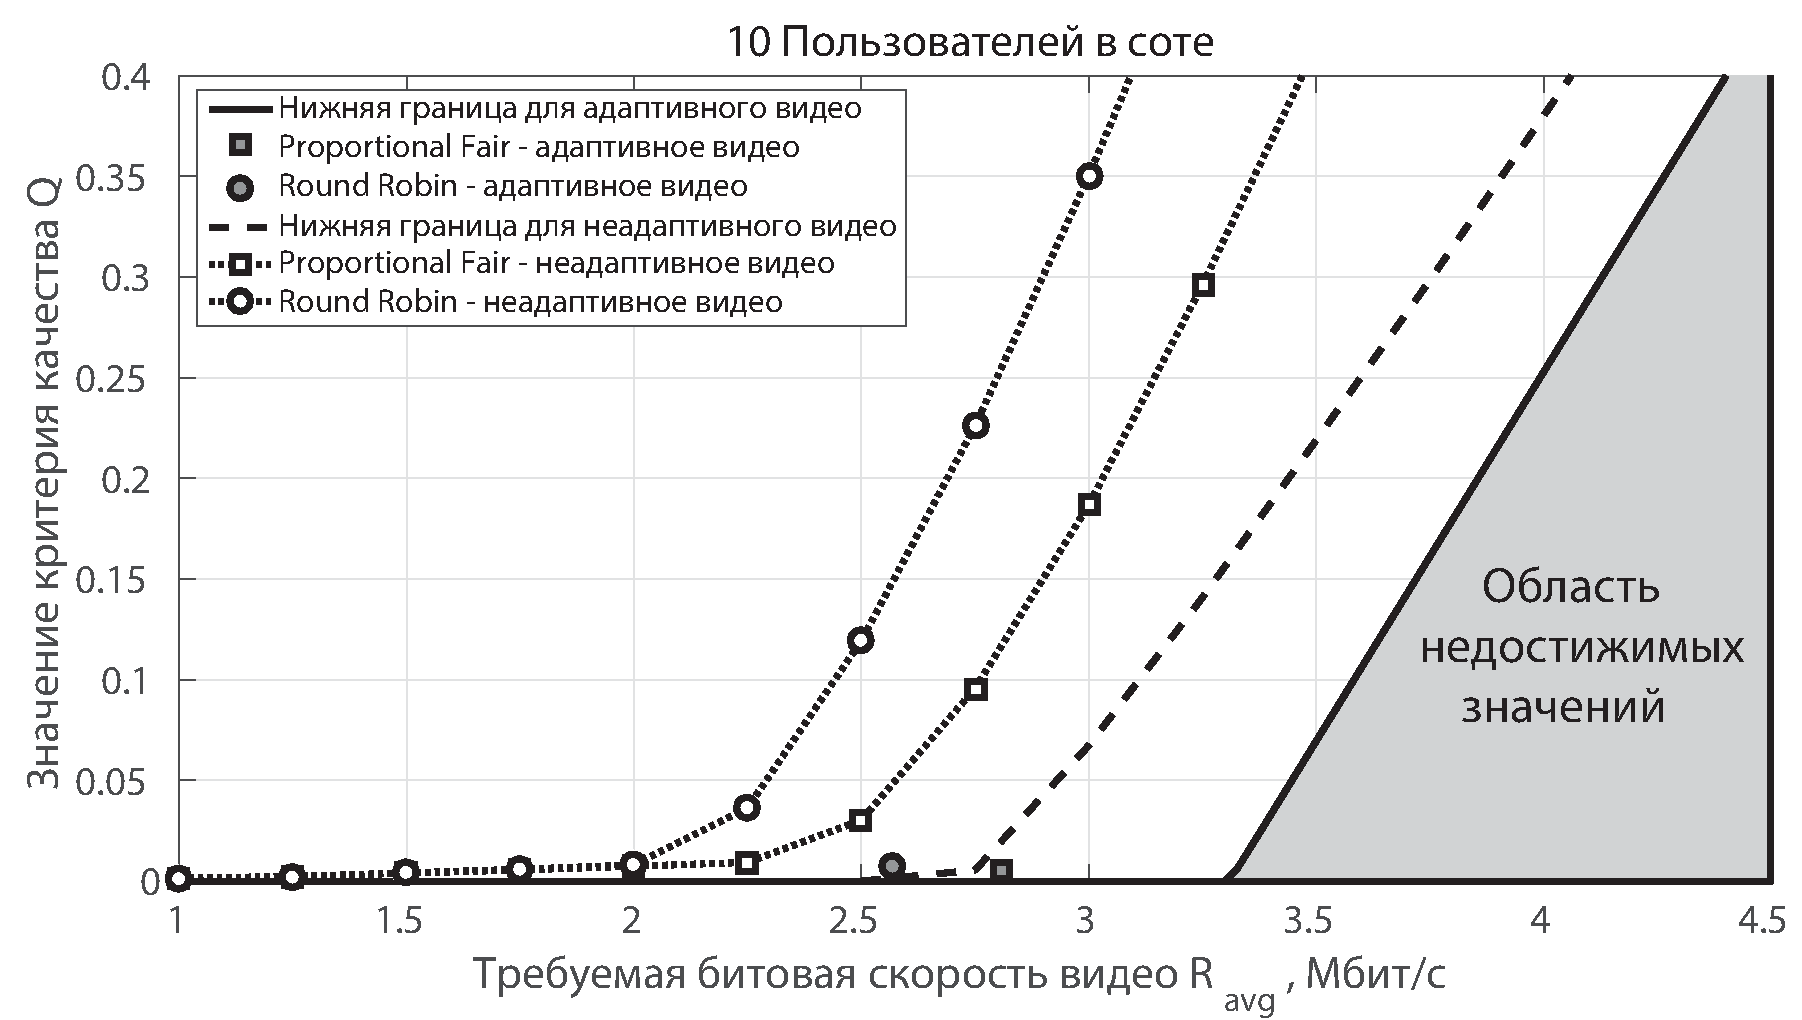
\includegraphics[width=\textwidth]{/Chapter4/10_Users_v2.pdf}
\caption{Сравнение производительности известных алгоритмов планирования при передаче адаптивного видео с нижней границей}
\label{fig:Q_PLOT}
\end{center}
\end{figure}

На рисунке \ref{fig:Users_cmp} представлено сравнение нижних границ для критерия $Q$ при наличии различного числа абонентов в соте. С ростом числа абонентов при заданном уровне значений критерия $Q$ система переходит в состояние перегрузки (определение \ref{def:Congestion}) при меньшем значении требуемой средней битовой скорости видеопотоков в соте.

\begin{figure}[htbp]
\begin{center}
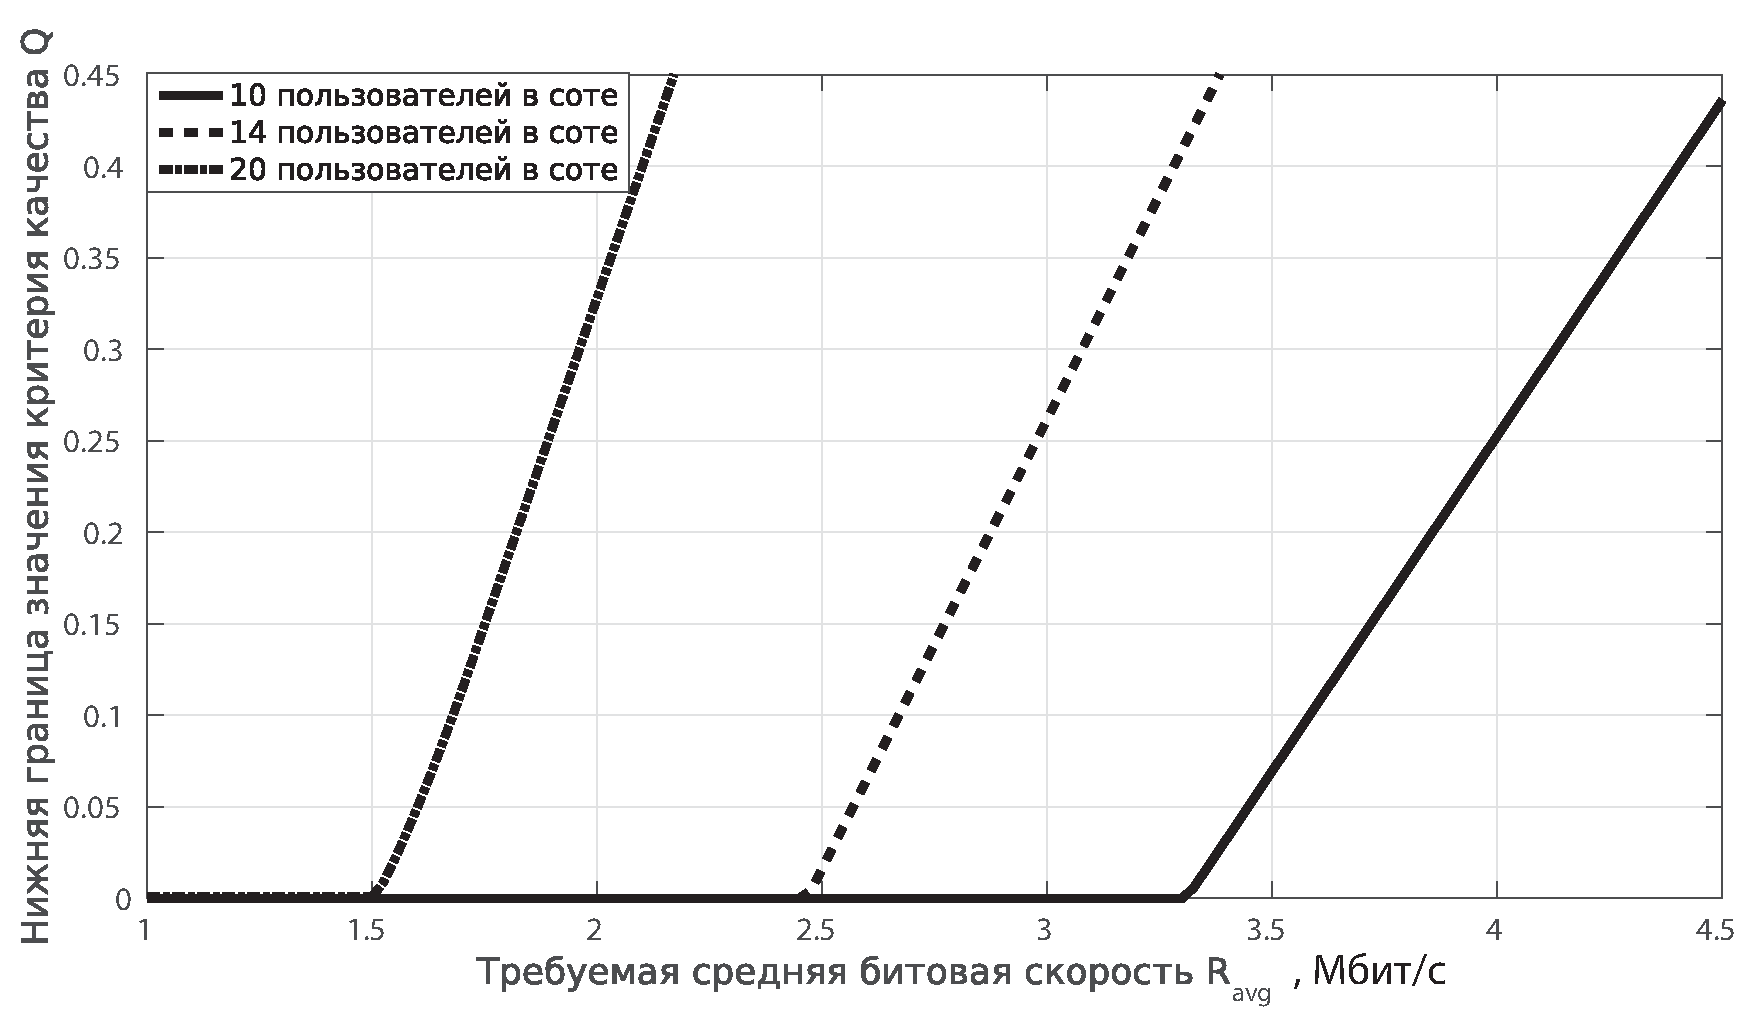
\includegraphics[width=\textwidth]{/Chapter4/Users_cmp.pdf}
\caption{Нижняя граница критерия $Q$ при различном числе абонентов в соте}
\label{fig:Users_cmp}
\end{center}
\end{figure}

Введем определение емкости соты:
\begin{definition}
\label{def:Capacity}
    \emph{Емкость соты}~--~число пользователей в соте, при котором значение критерия $Q$ равняется некоторой заданной величине.
\end{definition}
Определение \ref{def:Capacity} взаимосвязано с определеним перегрузки следующим образом: определение перегрузки задает границу значения критерия качества восприятия, при котором система перестает поддерживать требуемый уровень качества обслуживания. В свою очередь определение емкости соты определяет максимальное число пользователей, при котором система еще не перешла в состояние перегрузки.

Рисунок \ref{fig:capacity} иллюстрирует максимально возможную емкость соты для рассматриваемого сценария при значении критерия восприятия $Q$ равном $0.01$, $0.05$ и $0.1$ в зависимости от требуемой битовой скорости просматриваемых видеопотоков. Возможно отметить, что наибольшая емкость соты достигается при больших значениях критерия качетсва $Q$.

\begin{figure}[htbp]
\begin{center}
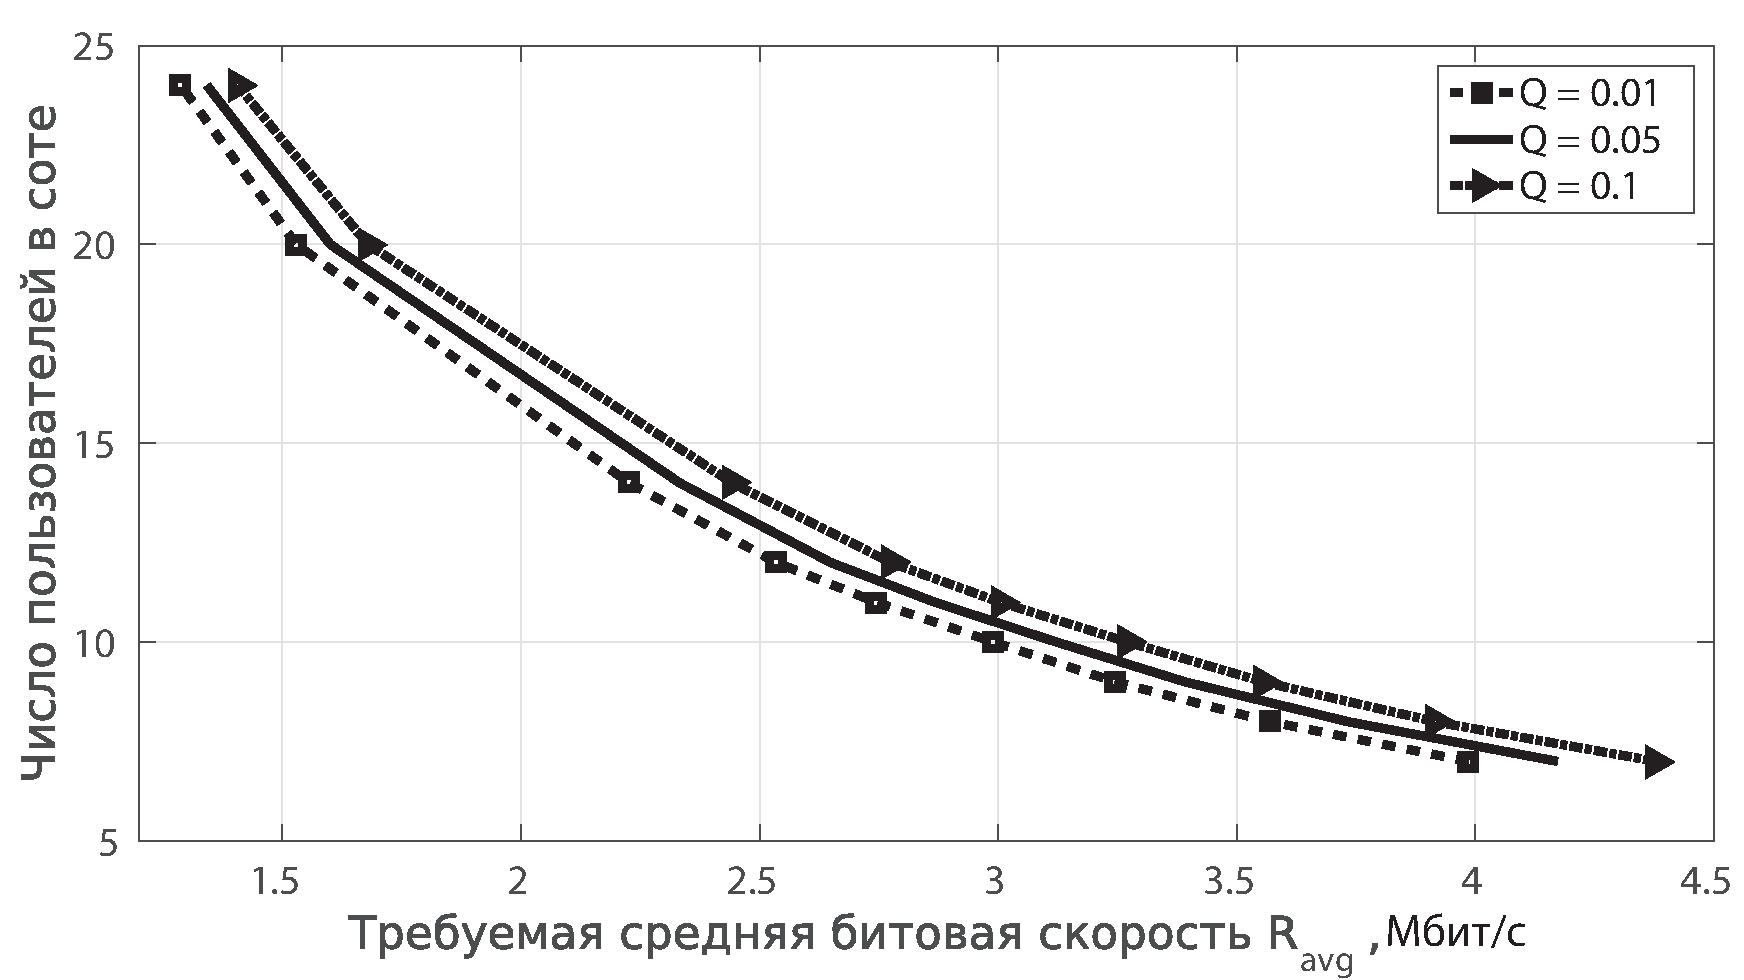
\includegraphics[width=\textwidth]{/Chapter4/capacity.pdf}
\caption{Максимальная емкость соты для различных значений критерия качества $Q$}
\label{fig:capacity}
\end{center}
\end{figure}

\section{Выводы по разделу}

В настоящем разделе была рассмотрена передача адаптивных видеопотоков по протоколу HTTP в беспроводных централизованных сетях связи. В начале раздела был предложен критерий качества восприятия адаптивного видео, учитывающий два основных фактора: длительность буферизации и битовая скорость просматриваемого видеопотока. На основе данного критерия была сформулирована оптимизационная задача невыпуклого программирования, определяющая максимально возможную производительность систем передачи данных для введенного критерия. Для поставленной оптимизационной задачи была найдена нижняя граница по всевозможным алгоритмам планирования распределения ресурсов беспроводного канала и адаптации видеопотока, удовлетворяющих допущениям, введенным в подразделе \ref{chap2:Assumptions}. В заключении раздела была продемонстрировано сравнение производительности существующих алгоритмов планирования с найденной нижней границей, и определена максимально возможная емкость соты для рассматриваемого сценария при передаче адаптивных видеопотоков.

В качестве результатов настоящего раздела могут быть выделены следующие:
\begin{itemize}
	\item Предложен критерий качества восприятия адаптивного видео: отношение длительностей буферизации и просмотра при ограничении снизу на среднее значение битовой скорости просматриваемого видеопотока (подраздел \ref{chap4:AdaptiveQoe});
	\item Для предложенного критерия произведена постановка оптимизационной задачи невыпуклого программирования. Для данной постановки найдена нижняя граница введенного критерия по всевозможным алгоритмам планирования и адаптации видеопотока, удовлетворяющих введенным допущениям в подразделе \ref{chap2:Assumptions}, с использованием двуступенчатой оптимизации (подразделы \ref{chap4:AdaptiveOptimizationProblem}, \ref{chap4:KktSolution} и \ref{chap4:LowerBoundForQ});
	\item Произведена демонстрация производительности существующих алгоритмов планирования в сравнении с найденной нижней границей и определена максимально возможная емкость соты для рассматриваемого сценария (подраздел \ref{chap4:NumericalExample}).
\end{itemize}

Настоящий раздел является заключительным в диссертационном исследовании и, для демонстрации общей картины проделанной работы, в приложении \ref{AppС} представлен граф основных зависимостей между подразделами (рисунок \ref{fig:graph_horizontal.pdf}). Нумерация узлов графа соответствует нумерации подразделов, направленные ребра (сплошные линии) обозначают прямые ссылки между подразделами (например, подраздел \ref{chap3:NonAdaptiveOptimizationProblem} ссылается на подразделы \ref{chap2:Assumptions} и \ref{chap2:InterrelationVideoParams}), пунктирные линии обозначают логическое соединение материалов подразделов.

Возможно отметить, что опорными подразделами настоящей работы являются \ref{chap2:Assumptions} и \ref{chap2:InterrelationVideoParams}, представляющие систему допущений и основополагающую взаимосвязь между характеристиками сети передачи данных и воспроизведением видеоряда соответственно. Основные результаты работы, представленные в подразделах \ref{chap2:InterrelationVideoParams}, \ref{chap3:LowerBoundForG} и \ref{chap4:LowerBoundForQ}, и их демонстрации \ref{chap3:NumericalExample} и \ref{chap4:NumericalExample}, непосредственно опираются на систему допущений (подраздел \ref{chap2:Assumptions}). Материалы подраздела \ref{chap2:Assumptions} сформированы на основе анализа передачи видео по протоколу HTTP (раздел \ref{chap1}) и современных беспроводных централизованных телекоммуникационных систем (подразделы \ref{chap2:WirelessSystemStructure}, \ref{chap2:RadioChannel} и \ref{chap2:Scheduler}).

Важным моментом проведенного исследования является связь между системой передачи видеоданных и замкнутой системой массового обслуживания с конечным числом абонентов (подраздел \ref{chap2:QueuningNetwork}). Из материалов подраздела \ref{chap2:QueuningNetwork} следует, что исследуемая система является обобщением замкнутой СМО с конечным числом абонентов, в которой каждая генерируемая заявка уникальна и длительности пауз между их отправками не являются экспоненциальными случайными величинами, а интенсивность обслуживания изменяется во времени и зависит от характеристик всего множества заявок, находящихся в буфере на обслуживающем устройстве. Настоящее диссертационное исследование предлагает новые аналитические результаты для подобных систем массового обслуживания.